\documentclass[border=2pt,tikz]{standalone}
\usepackage{tikz}
\usepackage{amsmath}
\usepackage{amssymb}

\begin{document}

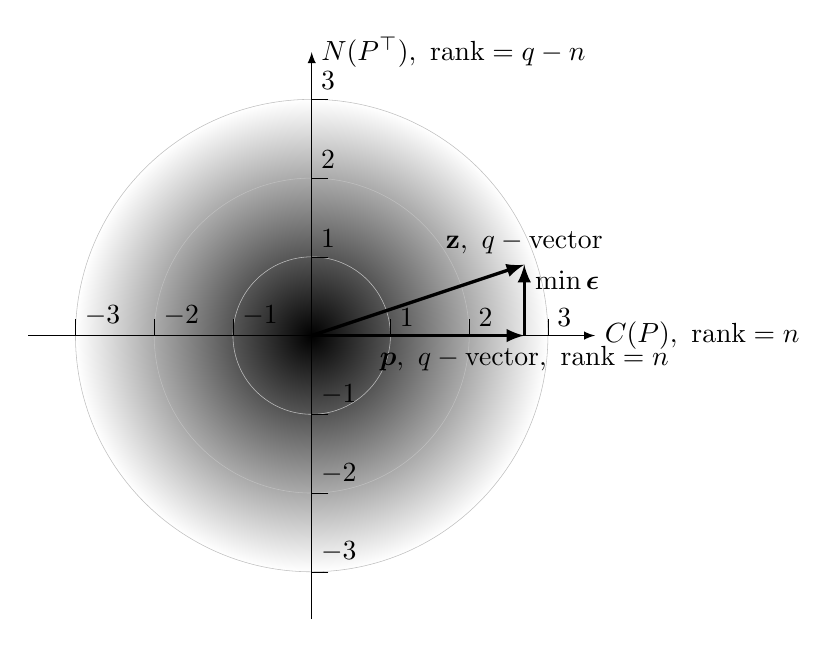
\begin{tikzpicture}[scale=3]

% Draw a circle at the origin of radius 1
\draw [very thin, lightgray, inner color=black!100, outer color=black!0] (0,0) circle (1);
\draw [very thin, lightgray] (0,0) circle (1/3);
\draw [very thin, lightgray] (0,0) circle (1/3*2);

% Draw x and y axis lines
\draw [->,>=latex] (-1.2,0) -- (1.2,0) node [right] {$C(P),\ \mathrm{rank}=n$};
\draw [->,>=latex] (0,-1.2) -- (0,1.2) node [right] {$N(P^{\top}),\ \mathrm{rank}=q-n$};

% 画标尺
\foreach \x in {-3, -2, -1, 1, 2, 3}
  \draw [very thin] (\x/3,2pt) -- (\x/3,0) node [above right] {$\x$};
\foreach \y in {-3, -2, -1, 1, 2, 3}
  \draw [very thin] (2pt,\y/3) -- (0,\y/3) node [above right] {$\y$};

\draw[very thick, ->,>=latex] (0.0, 0.0) -- (0.9, 0.3) node [above] {$\mathbf{z},\ q-\text{vector}$} ;
\draw[very thick, ->,>=latex] (0.9, 0.0) -- node [above right] {$\min \boldsymbol{\epsilon}$} (0.9, 0.3) ;
\draw[very thick, ->,>=latex] (0.0, 0.0) -- (0.9, 0.0) node [below] {$\boldsymbol{p},\ q-\text{vector},\ \mathrm{rank}=n$} ;

\end{tikzpicture}

\end{document}

